% 研制总结报告插图：输入状态机的两版画法（立项草图 / 重构后的完整状态机）
\documentclass[tikz,border=8pt]{standalone}
\usepackage{xeCJK}
\IfFontExistsTF{Noto Sans SC}
  {\setCJKmainfont{Noto Sans SC}}
  {\IfFontExistsTF{Source Han Sans SC}
    {\setCJKmainfont{Source Han Sans SC}}
    {\setCJKmainfont{Microsoft YaHei}}}
\usepackage{graphicx}
\usetikzlibrary{positioning,arrows.meta,calc,shapes.geometric}

\definecolor{ink}{HTML}{1F2937}
\definecolor{cblue}{HTML}{2563EB}
\definecolor{cgreen}{HTML}{059669}
\definecolor{corange}{HTML}{D97706}
\definecolor{cred}{HTML}{B91C1C}
\definecolor{cgray}{HTML}{6B7280}

\begin{document}
\begin{tikzpicture}[x=1cm,y=1cm,font=\small,
    st/.style={draw=#1!55!black, fill=#1!8, rounded corners=4pt, align=center,
      inner sep=3pt, text=ink, font=\small, line width=0.7pt,
      minimum height=1.30cm, minimum width=2.8cm},
    arr/.style={-{Latex[length=2mm]}, draw=ink!75, line width=0.8pt},
    lab/.style={font=\scriptsize, text=ink!85, inner sep=1.5pt},
    panel/.style={font=\small\bfseries, text=ink}
  ]

  % ================= （a）立项草图 =================
  \node[panel, anchor=west] at (0.3,12.78)
    {（a）10-15 立项草图：主线为“静止 → 预览 → 执行”三态};
  \node[inner sep=0pt] (sketch) at (7.9,9.70)
    {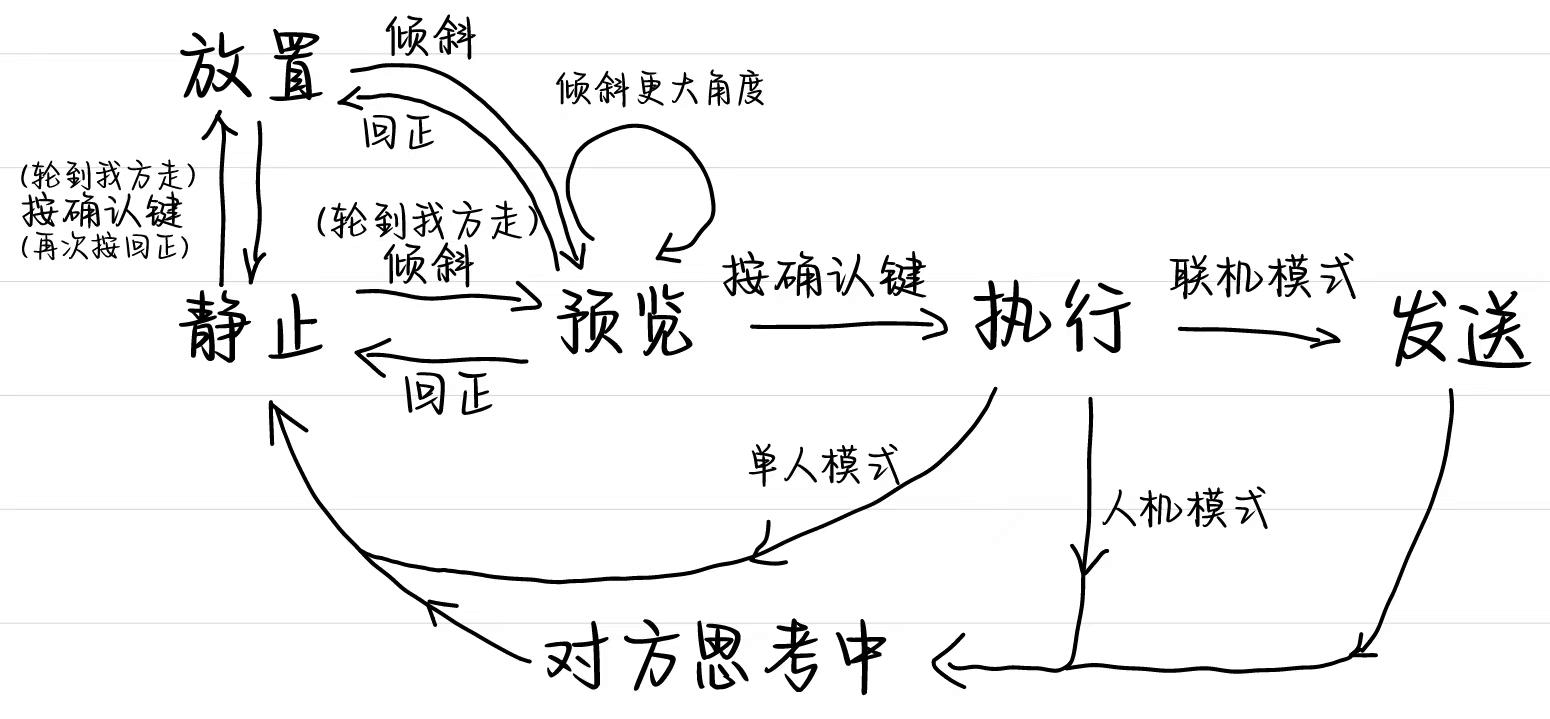
\includegraphics[width=12.4cm]{sketch-input.png}};

  % 分隔线
  \draw[dashed, draw=ink!25] (0.3,6.55) -- (15.5,6.55);
  \node[font=\scriptsize, text=cgray] at (7.9,6.76)
    {11-09 输入状态机重构（ADR-0009）：候选与可见选择分离、确认后锁定、补放兵分支};

  % ================= （b）重构后的状态机 =================
  \begin{scope}[yshift=3.55cm]
  \node[panel, anchor=west] at (0.3,2.20) {（b）重构后的完整状态机};

  % 状态
  \node[st=cblue] (idle) at (0,0) {\textbf{空闲}\\[0pt]\footnotesize 板子放平};
  \node[st=cblue] (cand) at (4.4,0) {\textbf{方向稳定中}\\[0pt]\footnotesize 候选未显示};
  \node[st=cblue] (prev) at (8.8,0) {\textbf{预览中}\\[0pt]\footnotesize 选择已显示};
  \node[st=corange] (done) at (13.0,0) {\textbf{已确认}\\[0pt]\footnotesize 等回中解锁};
  \node[st=corange] (place) at (0,-2.70) {\textbf{放兵模式}\\[0pt]\footnotesize 倾斜选格};

  % 主线
  \draw[arr] (idle.east) -- (cand.west);
  \node[lab] at (2.10,-0.32) {倾斜 $\ge 6^\circ$};
  \draw[arr] (cand.east) -- (prev.west);
  \node[lab] at (6.62,-0.32) {停稳 200 ms};
  \draw[arr] (prev.east) -- (done.west);
  \node[lab] at (11.00,-0.32) {按确认键};

  % 预览中：候选更新
  \draw[arr] (9.55,-0.58) .. controls (9.55,-1.55) and (7.55,-1.55) .. (8.15,-0.58);
  \node[lab, align=center] at (8.55,-1.90) {改方向 / 改数量\\再稳 200 ms 才更新};

  % 放兵模式
  \draw[arr, {Latex[length=1.6mm]}-{Latex[length=1.6mm]}]
    (idle.south) -- (place.north);
  \node[lab, align=left, anchor=west] at (0.20,-1.42)
    {金币足且有空位时\\按确认键落子或退出};

  % 回中总线
  \draw[draw=ink!75, line width=0.8pt] (cand.north) -- (4.4,1.45);
  \draw[draw=ink!75, line width=0.8pt] (prev.north) -- (8.8,1.45);
  \draw[draw=ink!75, line width=0.8pt] (done.north) -- (13.0,1.45);
  \draw[arr] (13.0,1.45) -- (0,1.45) -- (idle.north);
  \node[lab] at (6.40,1.62) {回中（$<4^\circ$ 持续 120 ms）：预览取消 / 解除锁定};
  \end{scope}

\end{tikzpicture}
\end{document}
